\section*{INTRODUCTION}\label{introduction}
The present dataset contains roll decay tests from actual model tests,
carried out at SSPA maritime-dynamics-laboratory (www.sspa.se) and also
CFD simulations, using a method called FNPF. The roll damping is
determined by identifying the roll damping parameters in a prescribed
mathematical model for the decaying roll motion. The roll angle time
series from a roll decay model test is shown in
Fig.\ref{fig:rolldecay_example}.
The analysis for this report can also be found at:
\begin{itemize}
\item GitHub: \url{https://github.com/martinlarsalbert/roll_decay_damping}
\item Binder: \url{https://mybinder.org/v2/gh/martinlarsalbert/roll_decay_damping/HEAD?filepath=reports%2Freport%2F01.1.report.ipynb}%2Freport%2F01.1.report.ipynb}%2F01.1.report.ipynb}
\end{itemize}
\begin{figure}[H]
\begin{center}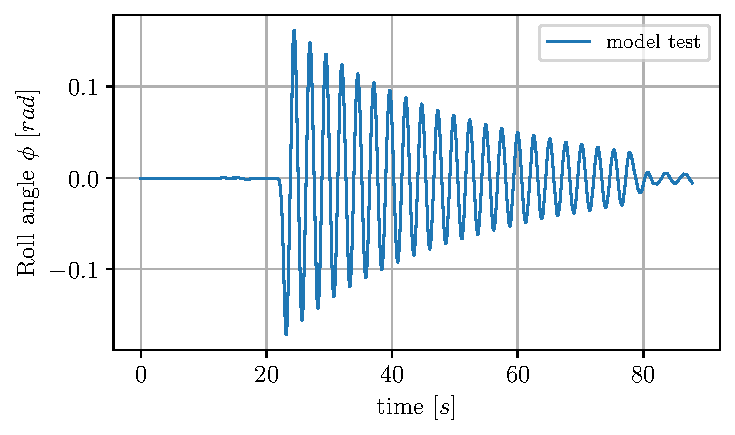
\includegraphics[width = 0.95\textwidth]{figures/rolldecay_example.pdf}\end{center}
\vspace{-0.7cm}
\caption{Roll decay time series}
\label{fig:rolldecay_example}
\end{figure}
The oscillating motion can be described by a spring-mass-damper system
as seen in Fig.\ref{fig:spring_mass_damper}.
\begin{figure}[H]
\begin{center}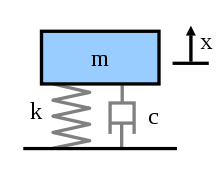
\includegraphics[width = 0.95\textwidth]{figures/spring_mass_damper.png}\end{center}
\vspace{-0.7cm}
\caption{Spring-mass-damper system}
\label{fig:spring_mass_damper}
\end{figure}
This system can me described as the following ordinary differential
equation:
\begin{equation}
A_{44} \ddot{\phi} + \operatorname{B_{44}}{\left(\dot{\phi} \right)} + \operatorname{C_{44}}{\left(\phi \right)} = 0
\label{eq:roll_decay_equation_general_himeno}
\end{equation}
Where $B_{44}(\dot{\phi})$ and $C_{44}(\phi)$ are the damping and
stiffness models. A cubic model can be obtained by using cubic damping:
\begin{equation}
\operatorname{B_{44}}{\left(\dot{\phi} \right)} = B_{1} \dot{\phi} + B_{2} \left|{\dot{\phi}}\right| \dot{\phi} + B_{3} \dot{\phi}^{3}
\label{eq:b44_cubic_equation}
\end{equation}
And cubic stiffness model:
\begin{equation}
\operatorname{C_{44}}{\left(\phi \right)} = C_{1} \phi + C_{3} \phi^{3} + C_{5} \phi^{5}
\label{eq:restoring_equation_cubic}
\end{equation}
The total equation is then written:
\begin{equation}
A_{44} \ddot{\phi} + \left(B_{1} + B_{2} \left|{\dot{\phi}}\right|\right) \dot{\phi} + \left(C_{1} + C_{3} \phi^{2} + C_{5} \phi^{4}\right) \phi = 0
\label{eq:roll_decay_equation_quadratic}
\end{equation}
This equation does not have one unique solution however. If all
parameters would be multiplied by a factor $k$ these parameters would
also yield as a solution to the equation. All parameters are therefore
divided by the total inertia $A_{44}$ (including added mass inertia),
replacing the parameters with new normalized parameters such as:
$B_{1A} = B_1/A_{44}$. The equation is now rewritten with these new
parameters which have unique solutions:
\begin{equation}
\left(B_{1A} + B_{2A} \left|{\dot{\phi}}\right|\right) \dot{\phi} + \left(C_{1A} + C_{3A} \phi^{2} + C_{5A} \phi^{4}\right) \phi + \ddot{\phi} = 0
\label{eq:roll_decay_equation_quadratic_a}
\end{equation}
